\subsection*{\textsf{\normalsize 2.8\hspace{0.5cm}ANALISIS PASAR}}
\addcontentsline{toc}{subsection}{2.8 ANALISIS PASAR}

Pengembangan PUSPA berpeluang menjadi perintis \textit{virtual personal assistant} maupun \textit{virtual friend}, di Indonesia. Teknologi yang diusung oleh PUSPA di antaranya adalah:
\begin{itemize}
	\item \textit{natural language processing},
	\item \textit{holoscreen} (\textit{surface computing}),
	\item \textit{augmented reality},
	\item dan \textit{ubiquitous computing},
\end{itemize}
yang paling tidak merupakan \textit{emerging technologies}.

Analisis yang dilakukan oleh lembaga riset \href{http://www.gartner.com}{Gartner} tentang ''\textit{Hype Cycle of Emerging Technologies}'' teknologi-teknologi di atas berada pada masa terobosan teknologi (\textit{technology trigger}). Gambar~\ref{fig:gartner} menunjukkan siklus Gartner yang dimaksud.

\begin{figure}
	\centering
		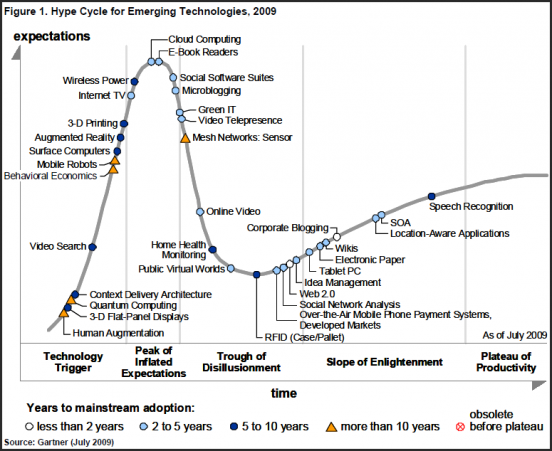
\includegraphics[scale=0.6]{gartner}
	\caption{Hype cycle of emerging technologies 2009 yang dipublikasikan oleh Gartner}
	\label{fig:gartner}
\end{figure}

Pada masa terobosan teknologi, pasar belum terpetakan dan \textit{market share} pun belum dibatasi. Sistem pemasarannya pun masih melalui pembahasan di media, demonstrasi publik di pameran-pameran, dan sebagainya. Kondisi ini adalah peluang besar untuk masuk ke pasar dan melakukan \textit{branding}.

Saat ini produk sejenis yang dapat berpeluang menjadi pesaing adalah produk Site Pal, dengan \textit{chatterbot} \href{http://alice.pandorabots.com}{A.L.I.C.E.}. Namun Site Pal adalah produk berbasis \textit{web}, sedangkan PUSPA berbentuk terminal.
Bagaimanapun, antarmuka \textit{web} untuk peran \textit{chatterbot} (tapi tidak untuk peran asisten) tetap dibuat untuk keperluan publikasi dan promosi.

Memasuki pasar pada masa terobosan teknologi memiliki kelemahan yaitu investasi pendidikan produk \textit{product knowledge} kepada masyarakat untuk memperbanyak pasar, sehingga target pasar PUSPA masih terbatas pada:
\begin{enumerate}
	\item museum,
	\item \textit{tenant} dan manajemen mal,
	\item perkantoran,
	\item dan aplikator rumah pintar,
\end{enumerate}
di mana kehadiran PUSPA secara umum diperlukan. Dengan target penjualan yang tidak terlalu tinggi, sepuluh saja per tahun, sudah dapat menghasilkan pendapatan usaha yang signifikan.

